Figure~\ref{fig:4:fw} in Chapter~\ref{chap:cc.fw} shows the structure of the
congestion control framework described in this thesis. The framework
categorizes \emph{In-path} sources and \emph{In-band} signaling for
implementing congestion control, which are discussed in this chapter. This
chapter is based on our work on congestion control for interactive multimedia
applications, which is documented in \citepub{c:3grc}, \citepub{c:hetrc},
\citepub{c:eval}, \cite{draft.xr.discard.rle}, \cite{draft.xr.bytes.discarded}
and \cite{Singh:control.loops.api}.

In \citepub{c:3grc}, we propose a new congestion control algorithm for the
mobile (e.g., 3G) environment, to be deployed in IP Multimedia System (IMS).
The main distinction between mobile (e.g., 3G, LTE) and other wireless
environments (e.g., 802.11x) is the media streams are transmitted using the
\emph{unacknowledged mode}; the packets corrupted due to bit-errors (e.g.,
wireless interference) are not re-transmitted and hence, packets incur low
delay. We compare a sender-driven congestion control with receiver-driven. In
\citepub{c:hetrc}, we extend the approach in \citepub{c:3grc} for deploying on
the Internet and show that the congestion control scheme is deployable.
Lastly, in \citepub{c:eval} we evaluate the performance of a congestion
control algorithm proposed by Google for WebRTC.

\section{Schemes of Congestion Control}

The congestion control algorithm can be implemented at the sender, at the
receiver, or co-operatively. The \emph{sender-driven} scheme requires that the
receiver measures the current network conditions and signals these congestion
cues to the sender which calculates the new sending rate (sender's estimate)
and uses it as the new sending rate. In the \emph{receiver-driven} scheme, the
receiver calculates the new sending rate (receiver's estimate) based on the
congestion cues, and signals the new rate to the sender, which on receiving
the new rate, adapts the media bit rate. In the \emph{co-operative} scheme,
the receiver calculates the new rate but along with the new rate also signals
the congestion cues, the sender calculates its new rate based on its
congestion cues and chooses a new sending rate between its estimate and the
receiver's estimate. Figure~\ref{fig:cc:scheme} shows the interaction of the
sender and receiver for each scheme.

\begin{figure}
  \centerline{
    \subfloat[Sender-driven Scheme]{
      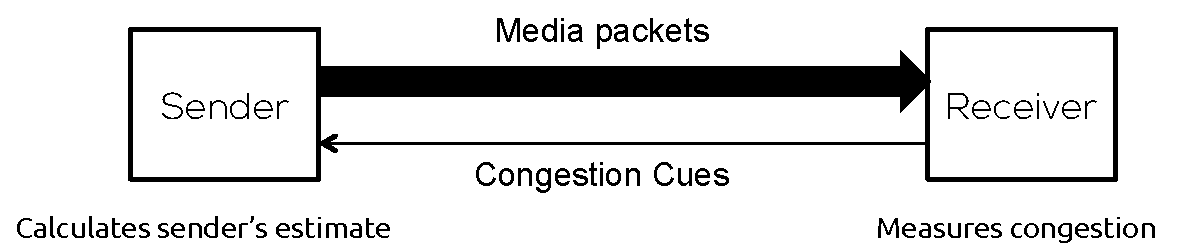
\includegraphics[width=\textwidth]
      {chap5-fig-cc-scheme-s}
    }
  }
  \centerline{
    \subfloat[Receiver-driven Scheme]{
      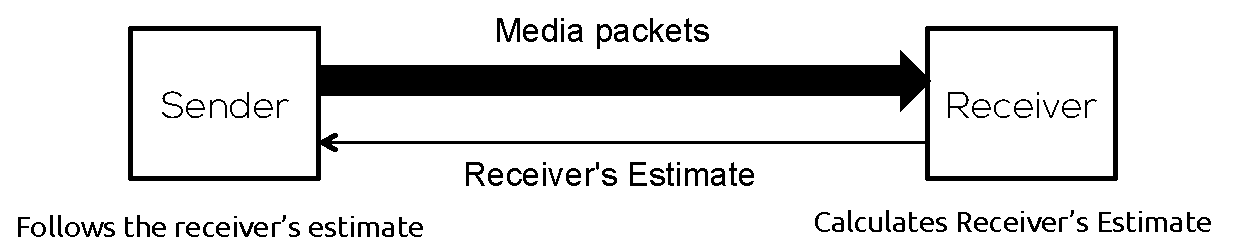
\includegraphics[width=\textwidth]
      {chap5-fig-cc-scheme-r}
    }
  }
  \centerline{
    \subfloat[Co-operative Scheme]{
      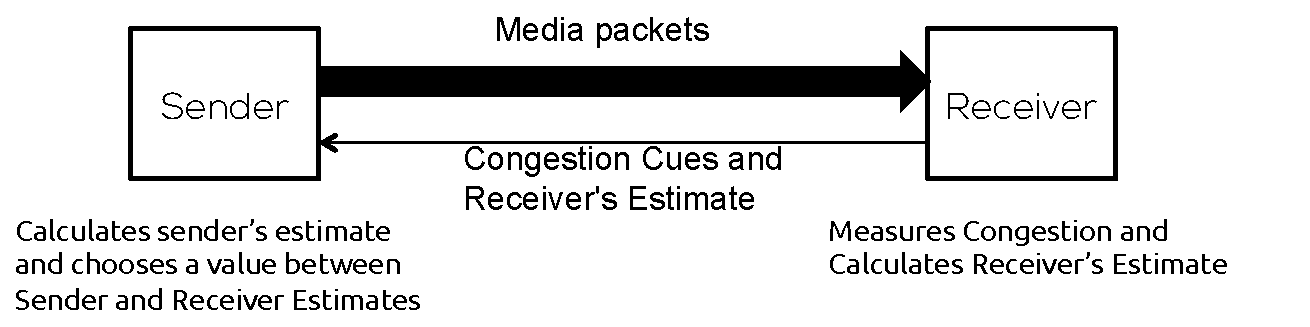
\includegraphics[width=\textwidth]
      {chap5-fig-cc-scheme-c}
    }
  }
  \caption{Congestion control schemes a) sender-driven, b) receiver-driven
and c) co-operative.}
  \label{fig:cc:scheme}
\end{figure}


\subsection{Sender-driven Congestion Control Scheme}

TCP Friendly Rate Control (TFRC) is an equation based congestion control
algorithm implemented at the sender~\cite{tfrc_347397} and is also implemented
as a profile~\cite{rfc4342} in the Datagram Congestion Control Protocol
(DCCP)~\cite{rfc4340}. TFRC uses the average packet size, RTT,
loss-rate~\cite{rfc3448} to calculate the new sending rate.
\cite{draft.rtp.tfrc} maps the timing rules defined in~\cite{rfc4828, rfc5348}
to that of RTP/RTCP feedback loop, it also redefines the timing rules in
AVPF-profile~\cite{rfc4585} for very short RTTs ($<20ms$).
\cite{Gharai06:ICME} shows that TFRC is stable on large RTT paths but less
stable for shorter paths~\cite{saurin:2006:thesis}. Our results in
\citepub{c:3grc} shows that TFRC underutilizes the link (average bandwidth
utilization (ABU) is between 30-40\%) and has higher fractional loss (\~6\%)
which results in lower PSNR. Figure~\ref{fig:tfrc} shows the performance of
TFRC on a slow time-varying link and a 3G link.

\begin{figure}
  \centerline{
    \subfloat{
      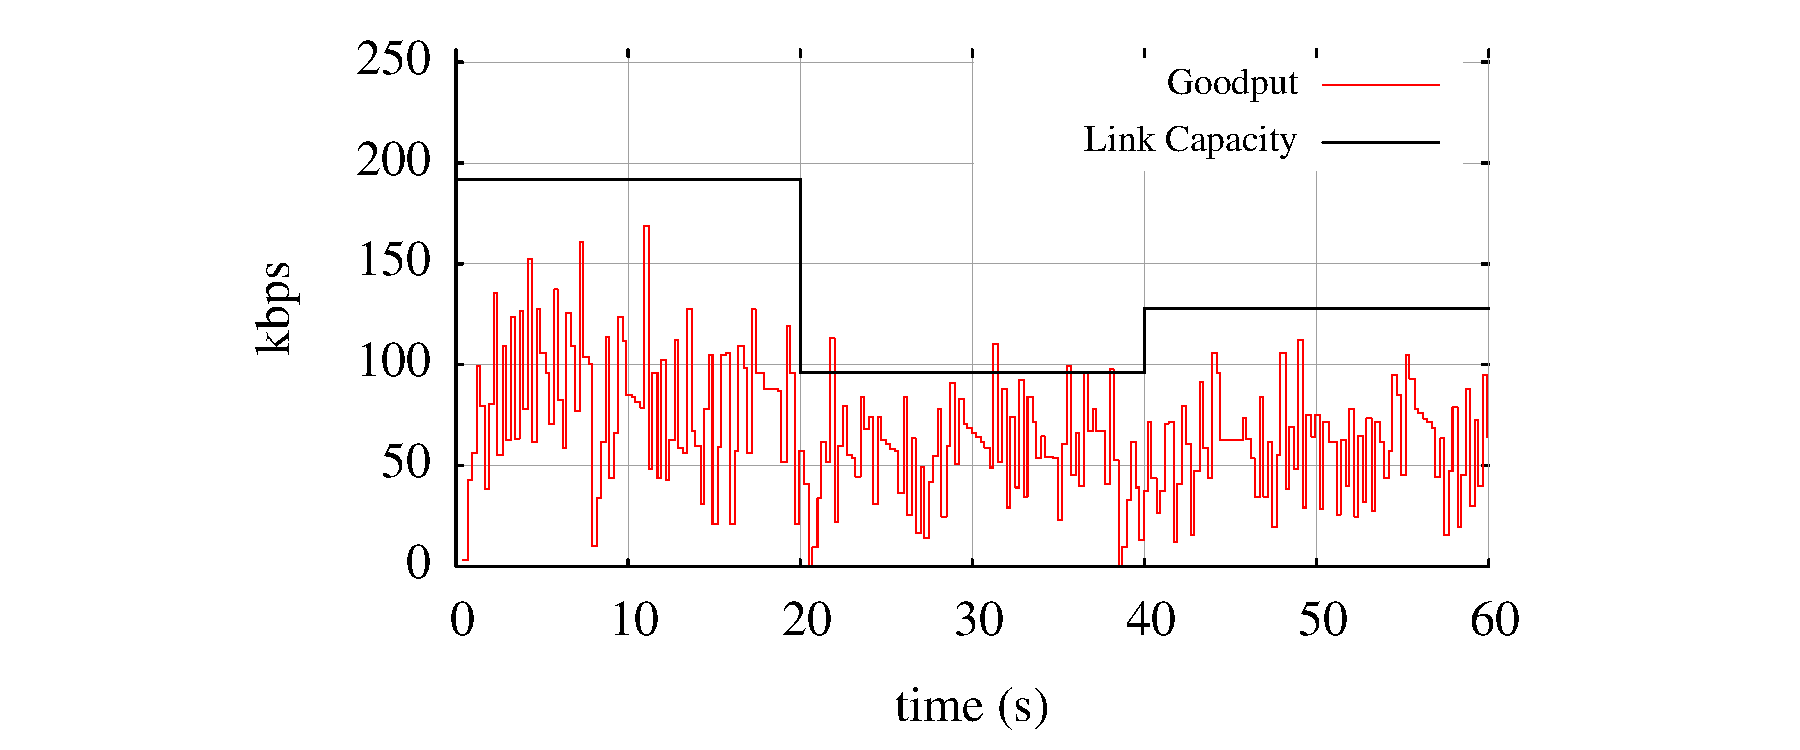
\includegraphics[width=0.6\textwidth, clip=true, trim=2cm 0 4cm 0]
      {chap5_graph_sl_tfrc}
    }
    \subfloat{
      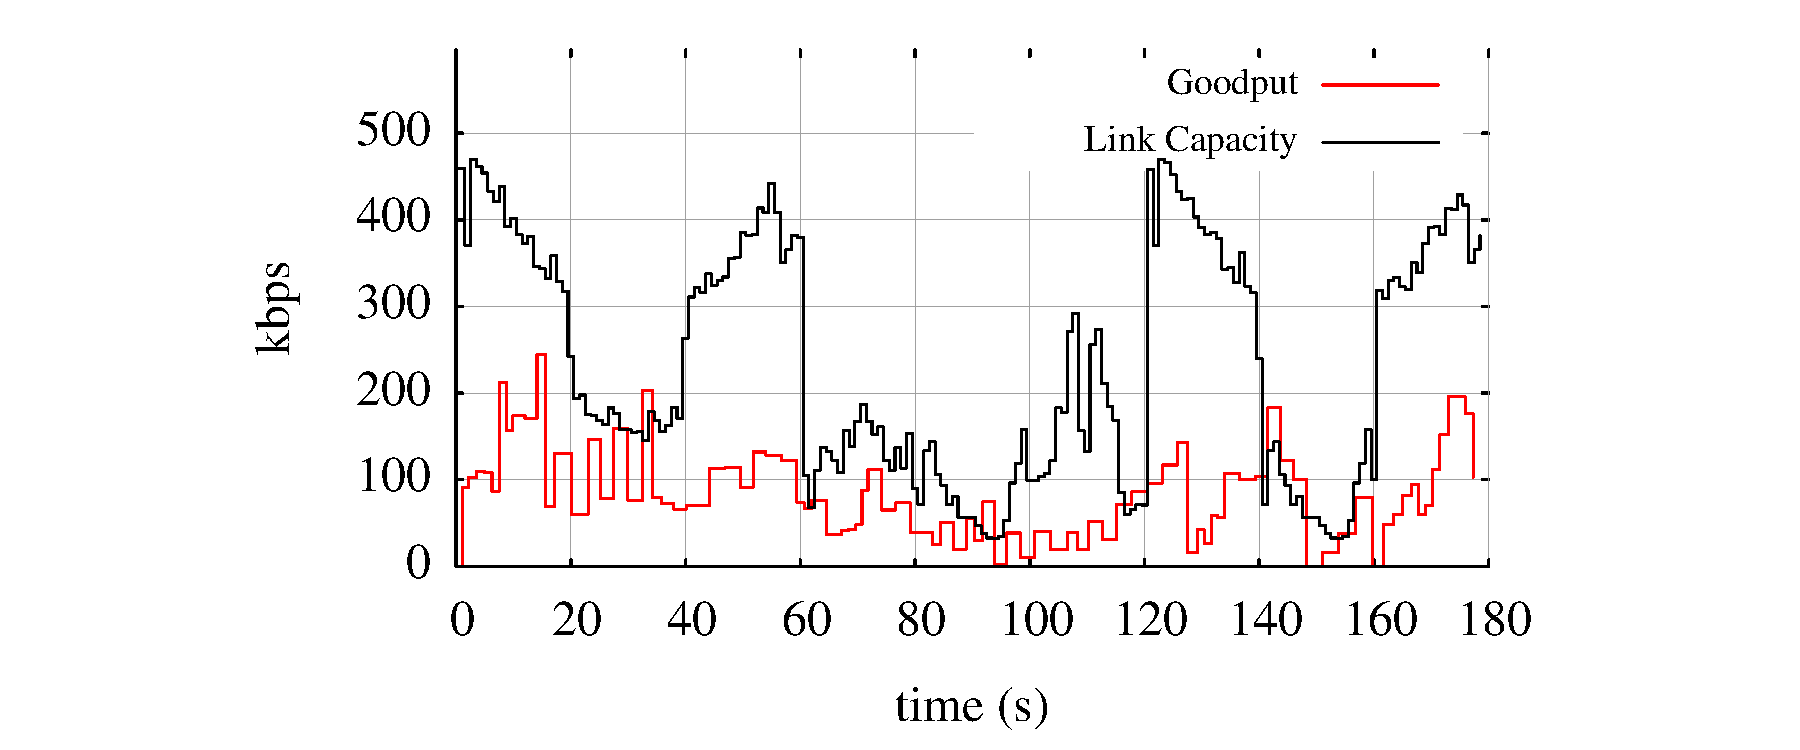
\includegraphics[width=0.6\textwidth, clip=true, trim=2cm 0 4cm 0]
      {chap5_graph_3g_tfrc_1}
    }
  }
  \caption{Performance of TFRC in a slow time-varying link and 3G network.}
  \label{fig:tfrc}
\end{figure}


\subsection{Receiver-driven Congestion Control Scheme}

Temporary Maximum Media Bit-rate Request (TMMBR) is defined as a codec control
messages in \cite{rfc5104}, it is generated by the receiver in a
point-to-point video call. The receiver calculates new estimate based on the
average inter-arrival time of RTP packets (\emph{video frames}) between two
RTCP RRs. The TMMBR indicates to the sender to limit its maximum sending rate
to the value requested in the message. Our results in \citepub{c:3grc} shows
that TMMBR-based congestion control utilizes the link better than TFRC (ABU
between 50-70\%) and much lower fractional loss ($\le$2\%).
Figure~\ref{fig:tmmbr} shows the performance of TMMBR on a slow time-varying
link and a 3G link.

\begin{figure}
  \centerline{
    \subfloat{
      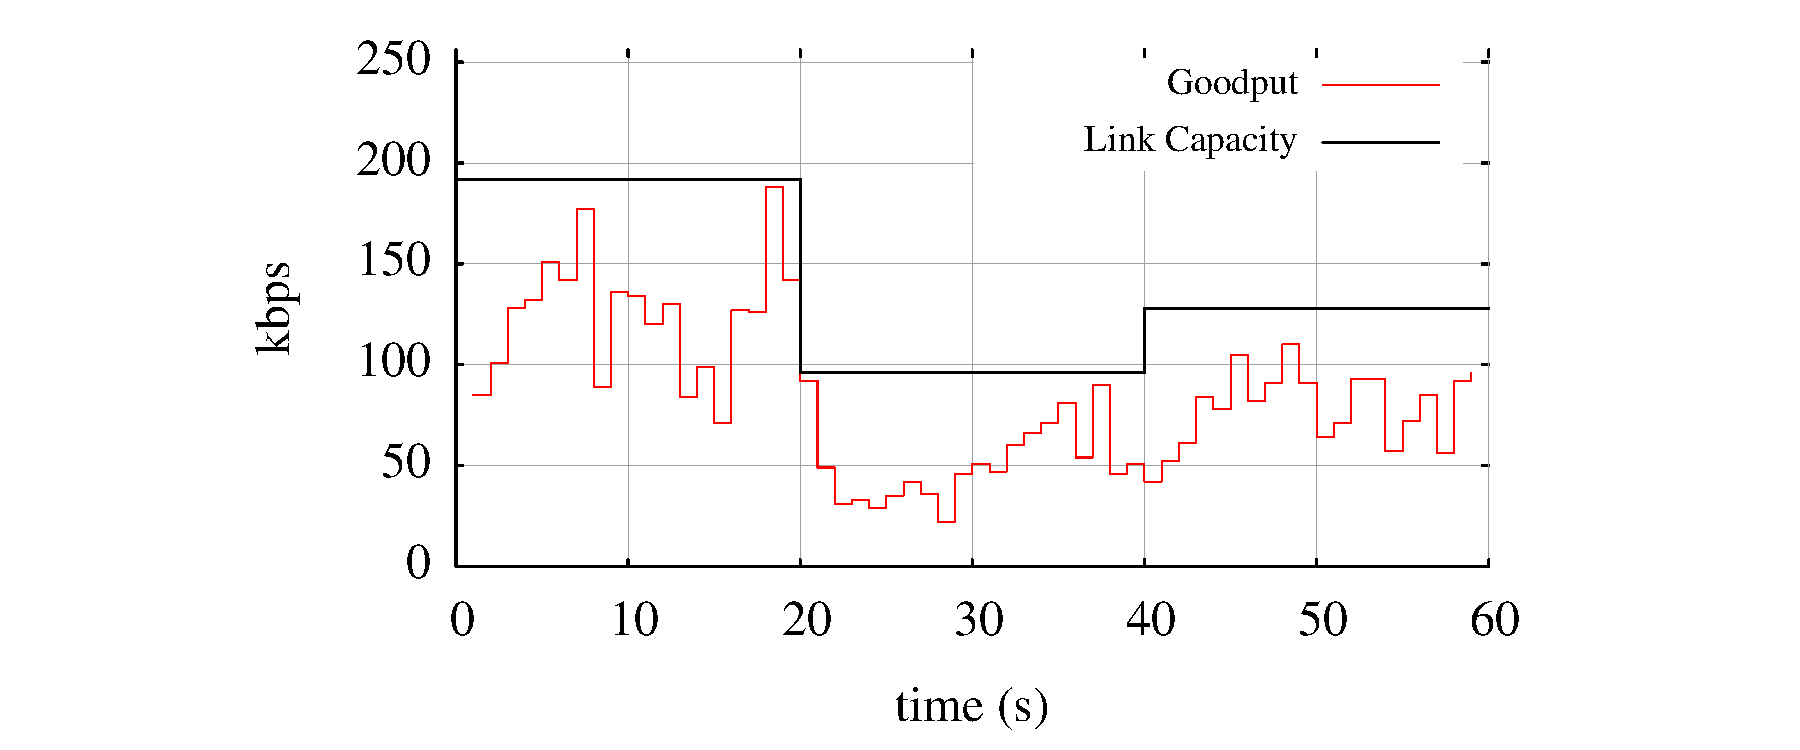
\includegraphics[width=0.6\textwidth, clip=true, trim=2cm 0 4cm 0]
      {chap5_graph_sl_tmmbr}
    }
    \subfloat{
      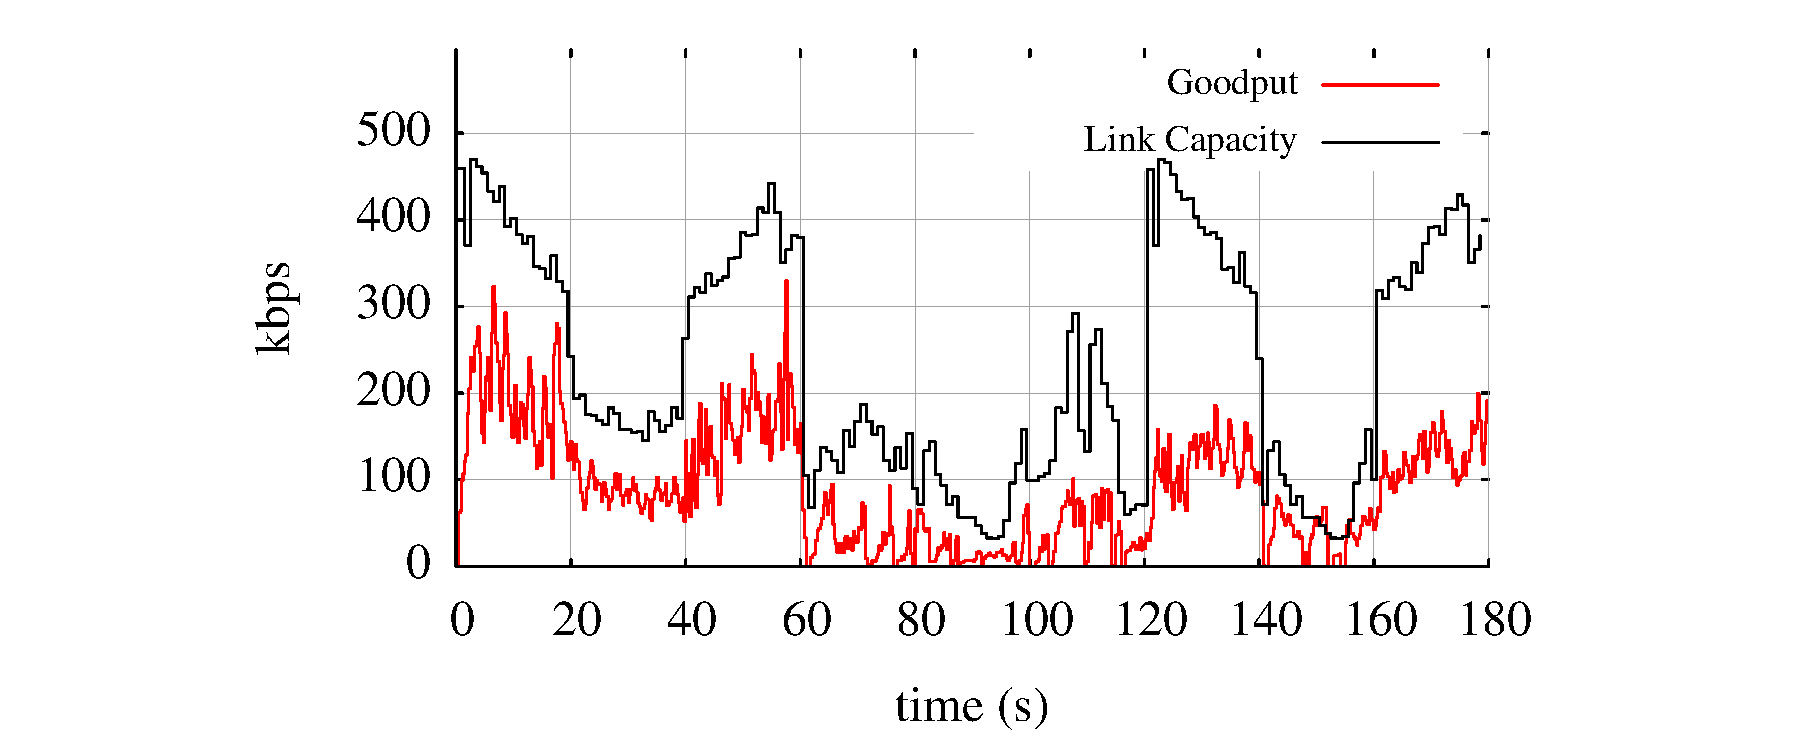
\includegraphics[width=0.6\textwidth, clip=true, trim=2cm 0 4cm 0]
      {chap5_graph_3g_tmmbr_u}
    }
  }
  \caption{Performance of TMMBR in a slow time-varying link and 3G network.}
  \label{fig:tmmbr}
\end{figure}

\subsection{Co-operative Congestion Control Scheme}

Conversational NADU (C-NADU) described in \citepub{c:3grc} is an extension to
Next Application Data Unit (NADU) signaling for video
streaming~\cite{nadu.1070341,nadu.1530486}. A NADU receiver measures the
playout delay and signals it to the sender along with the next sequence number
to be played out. In C-NADU, the receiver also calculates the \emph{receiver
estimate} by measuring the frame inter-arrival time and signals that along
with the NADU report. At the sender, the application calculates the
TCP-friendly rate,

\begin{figure}
  \centerline{
    \subfloat{
      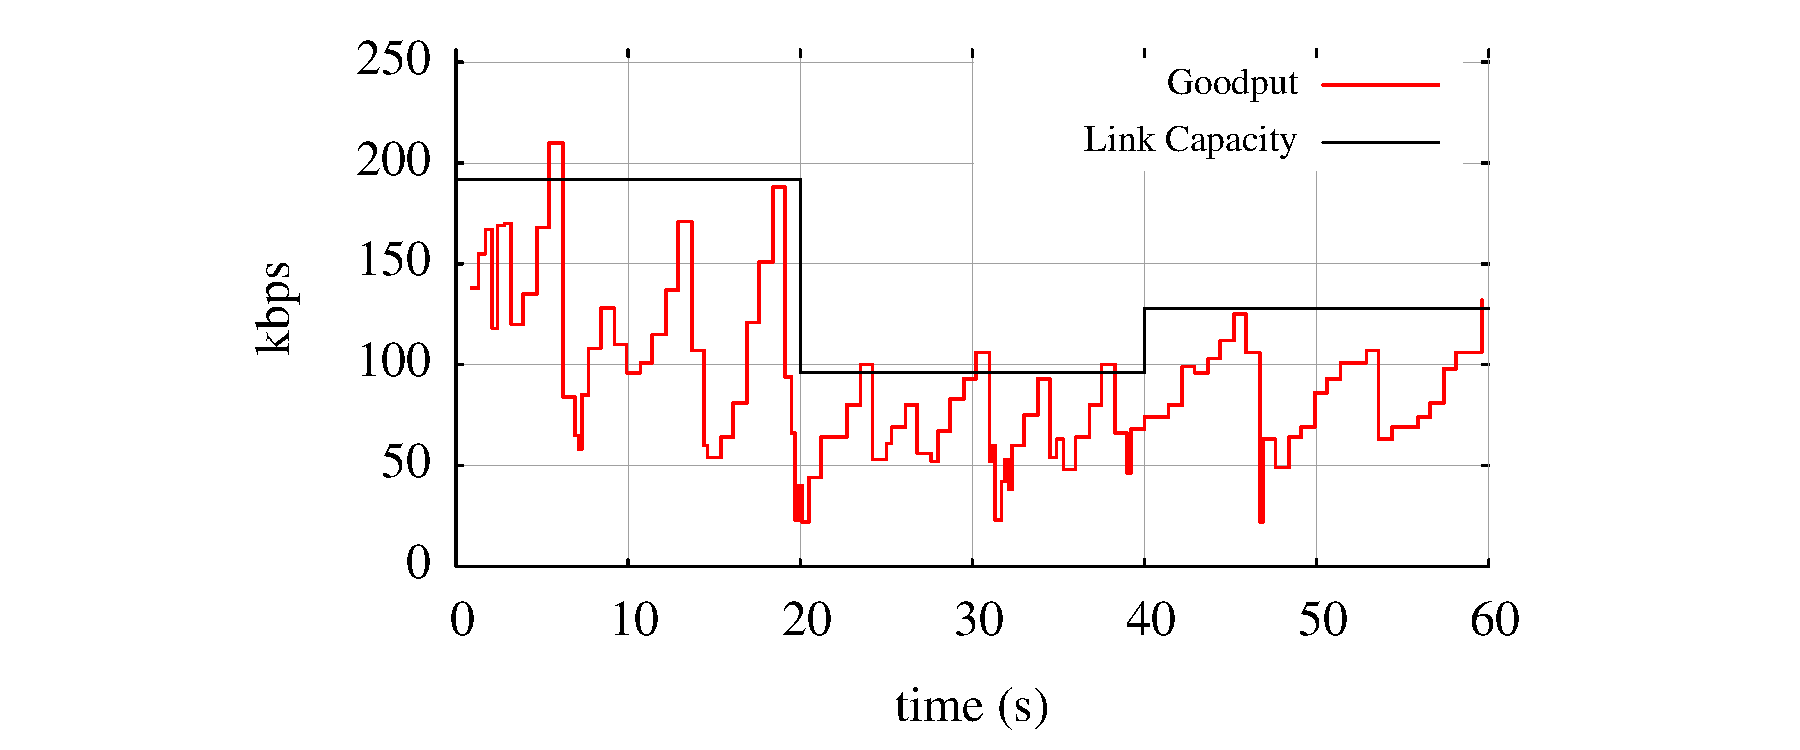
\includegraphics[width=0.6\textwidth, clip=true, trim=2cm 0 4cm 0]
      {chap5_graph_sl_cnadu}
    }
    \subfloat{
      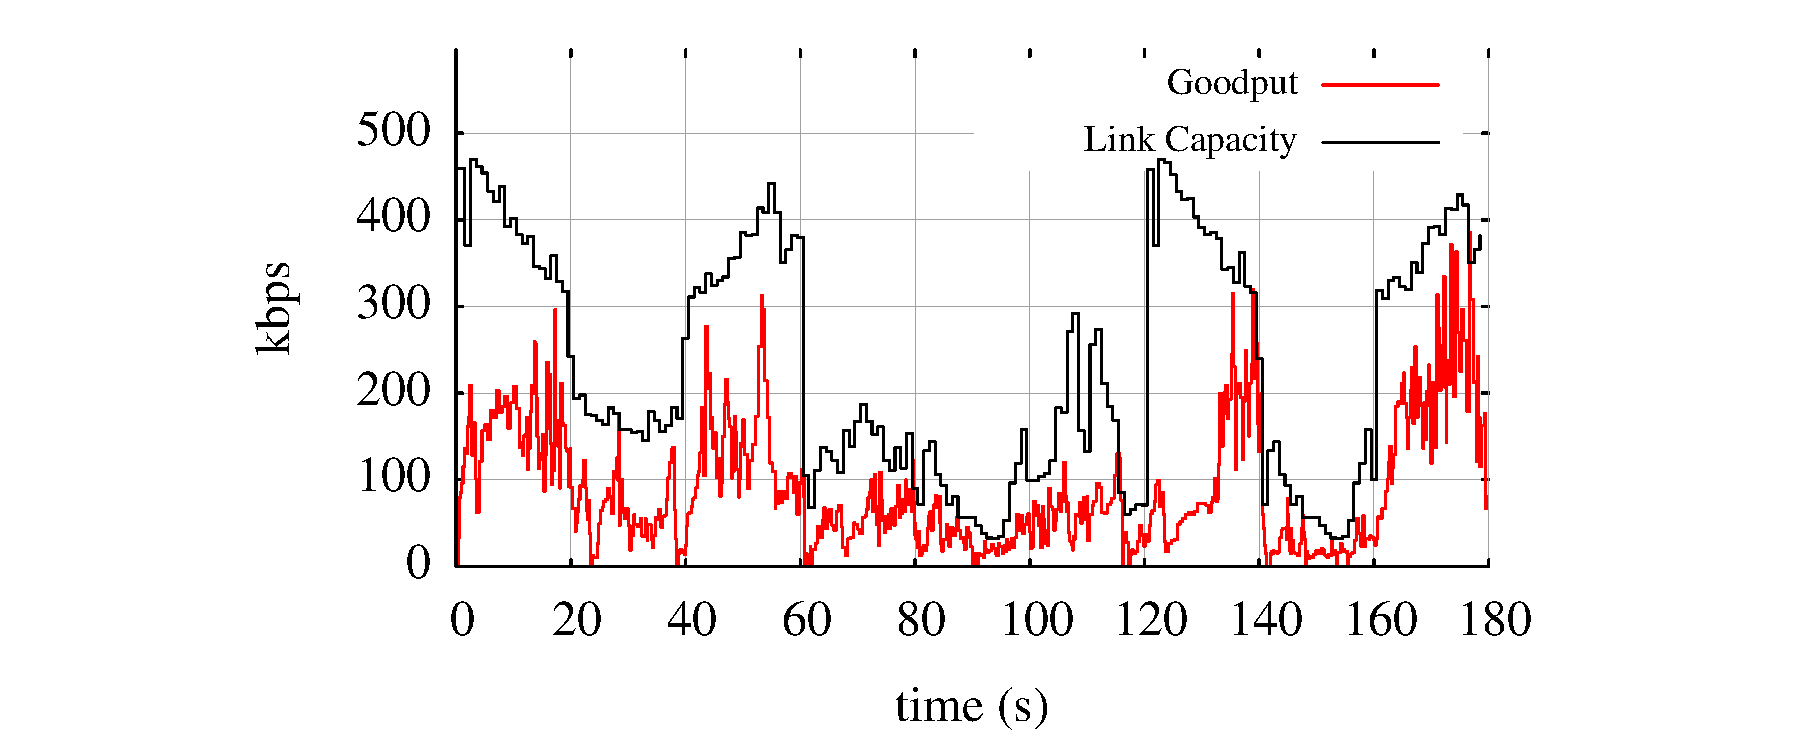
\includegraphics[width=0.6\textwidth, clip=true, trim=2cm 0 4cm 0]
      {chap5_graph_3g_cnadu}
    }
  }
  \caption{Performance of TMMBR in a slow time-varying link and 3G network.}
  \label{fig:cnadu}
\end{figure}